\cia
\vspace{-2.5cm}
\section{Vertex correction and cut} 
\label{sec:vertexcorr}
For each track found with the reconstruction code, a vertex $(x,y,z)$ is calculated
from the intersection of that track with the midplane\footnote{The midplane 
of a sector is defined by the plane that divide that sector in half and contains the beamline $(0,0,z)$.}  
of the corresponding sector.
If during the experiment the beam was not centered at $(0,0)$ an offset is introduced 
in the vertex calculation.

During the e1-6 running period  
the beam was not centered at $(0,0)$ and an  offset was introduced
in the vertex calculation as 
one can see in \F{fig:vertex_id}, where the events on the window\footnote{A window was placed at $z=+0.5$ cm
to help these kind of studies and to be a z-position reference.}
downstream of the target were selected to fix the z position as reference.

\begin{figure}[h]
 \begin{center}
  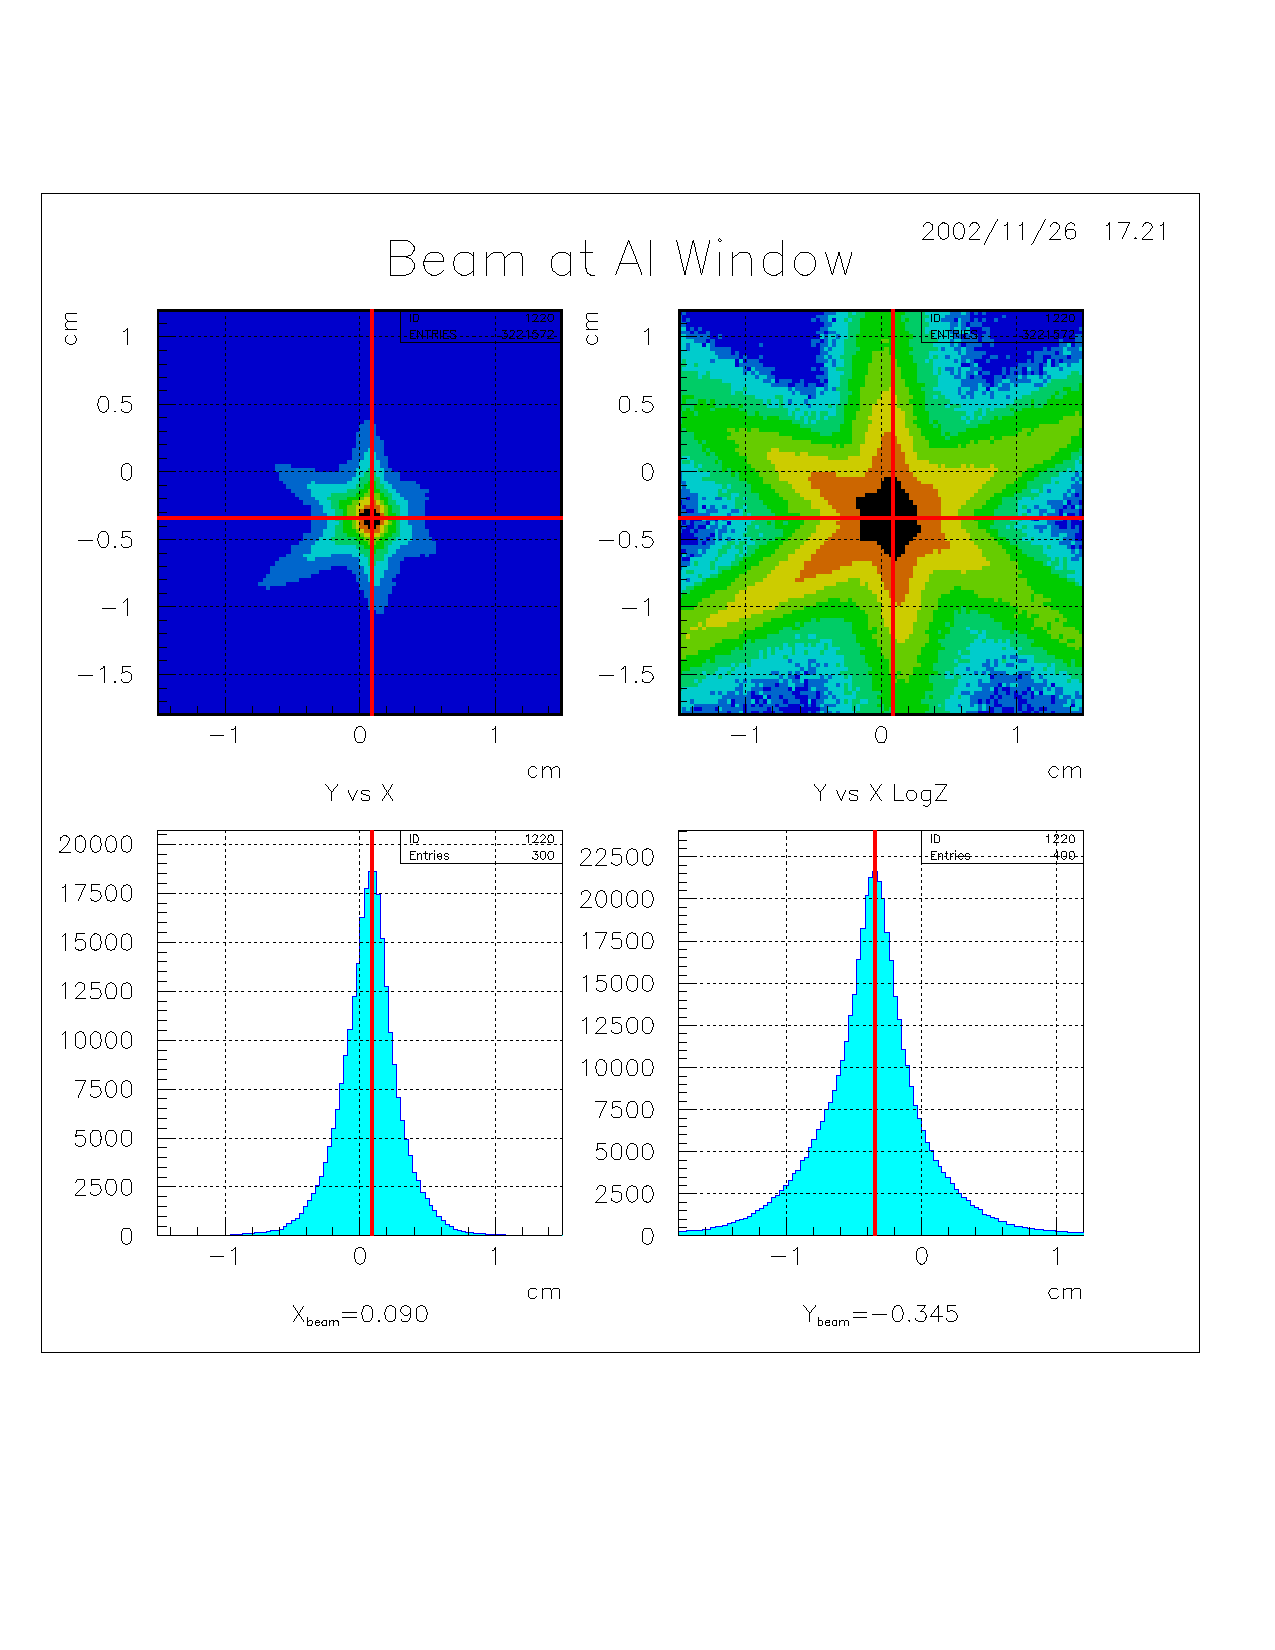
\includegraphics[width=11cm, bb=0 120 680 720]{data_reduction/img/vertex_id}
  \caption[ x and y position of the vertex at the window]
          {  Top: y versus x position of the vertex at the window. Upper right: same as upper left, 
	              except plotted logarithmically.
	              One can see that the beam spot
                      was slightly shifted from $(0,0)$. Bottom: the x (left) and y (right) 
		      distributions which led to the $x_0$ and $y_0$ calculation. }
 \label{fig:vertex_id}
 \end{center}
\end{figure}


\cia
The obtained values \cite{bib:valeri2}  for the beam position are:
$$
\begin{array}{c c c}
 x_0 = & 0.090   & cm \\
 y_0 = & -0.345 & cm
\end{array}
$$



To correct the vertex position it is sufficient to shift the midplanes 
so that they contain the correct beamline $(0.09, -0.345, z)$ and recalculate the intersection of the tracks
with the new planes. 
This is illustrated in \F{fig:vertex}.

\begin{figure}[h]
 \begin{center}
  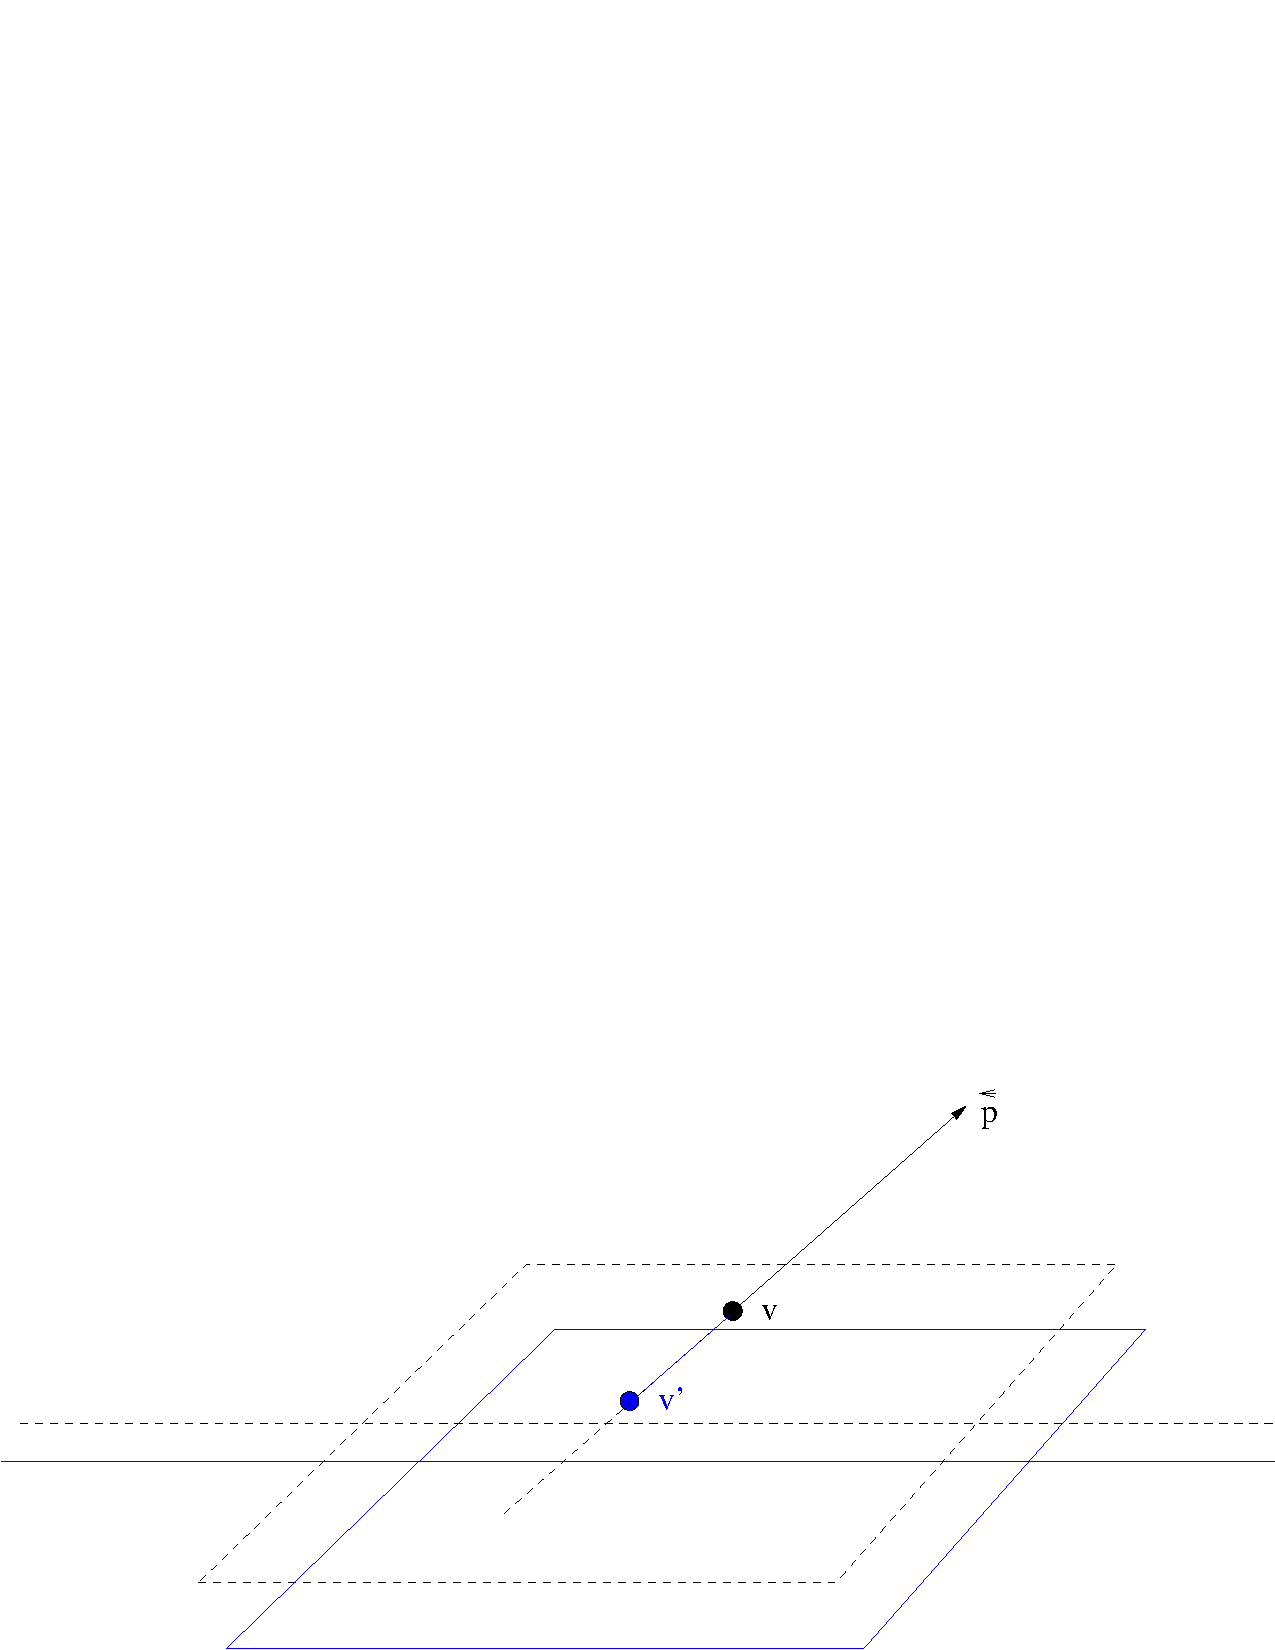
\includegraphics[width=11cm, bb=50 -30 650 360]{data_reduction/img/vertex}
  \caption[The vertex correction]
          { The vertex correction. The dashed plane is the original midplane containing 
	             the wrong beamline $(0, 0, 0)$. The point $v$ is the intersection of the track 
		     (straight line along momentum $\vec p$) with this plane.
		     The solid blue plane represents the corrected midplane containing $(0.09, -0.345, z)$.
		     The correction algorithm simply intersects the same track with the corrected 
		     midplane.}
 \label{fig:vertex}
  \end{center}
\end{figure}
\cia
The effect of the correction on the electron z position sector by sector is shown in \F{fig:vertex_corr}.

\begin{figure}[h]
 \begin{center}
  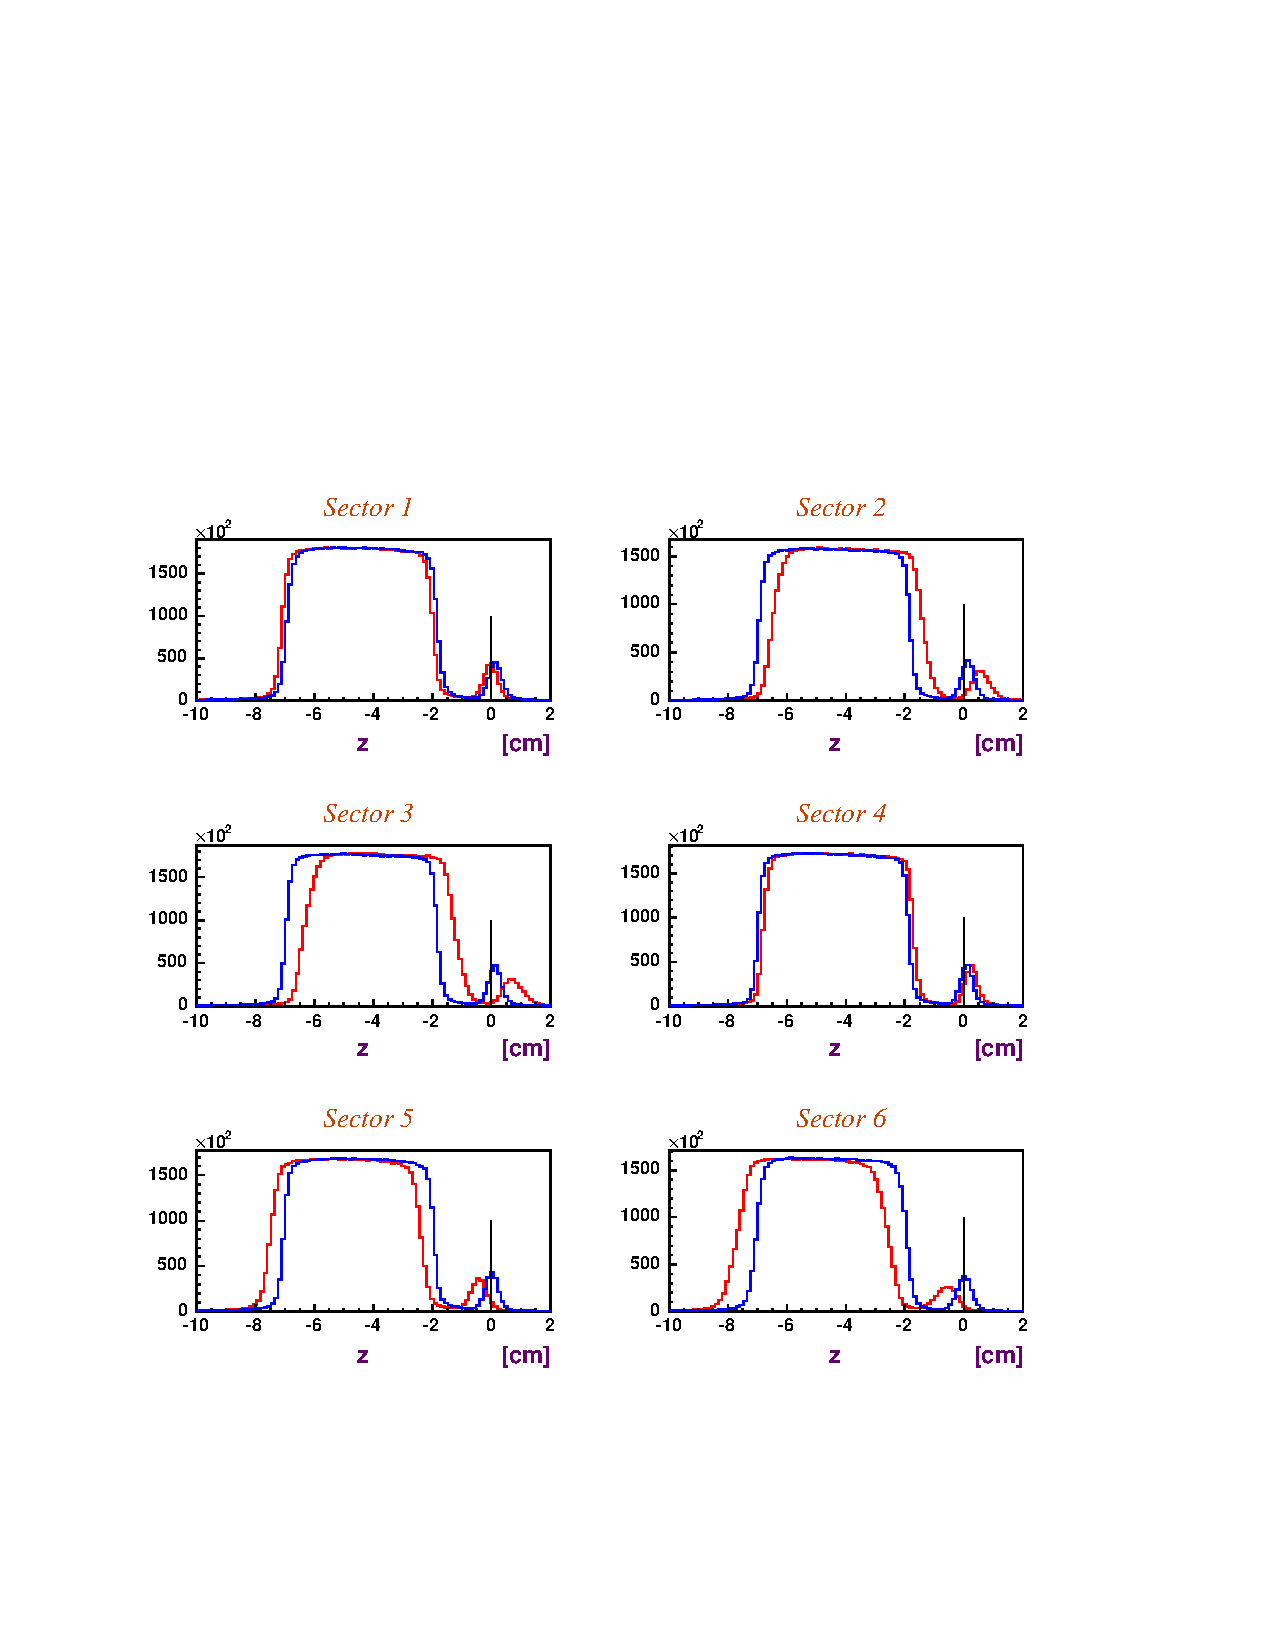
\includegraphics[width=11cm, bb=60 120 520 620]{data_reduction/img/vertex_corr}
  \caption[The vertex correction effect on electron z distributions for each sector]
          { The vertex correction effect on electron z distributions for each sector. 
	             Blue: before correction. Red: 
                     after correction. The corrected distributions are alligned with each other
                     and the resolution is improved as one can see looking at the 
                     window events. 
                     Similar effects on the other particles are observed.}
 \label{fig:vertex_corr}
   \end{center}
\end{figure}
The vertex resolution at this point is good enough to introduce a cut on the z vertex of electron and protons
in order to select events inside the target cell as follows:
\begin{equation}
 -8\, cm \le z \le -0.8\, cm
\label{eqn:vertex_cut1} 
\end{equation}

Furthermore the electron and proton vertices are required to be coincident along the $z$ axis
within the reconstruction resolution, so
an additional cut on $\Delta z = z_{electron} - z_{proton}$ ensures that the electron and proton 
$z$ vertex positions lie within $1.6$ cm:

\begin{equation}
 \left| \Delta z \right| < 1.6 \,cm
 \label{eqn:vertex_cut2} 
\end{equation}

\F{fig:vertex_cut} illustrates the effect of the vertex correction on $\Delta z$ 
integrated over all sectors and
both the \ref{eqn:vertex_cut1} and \ref{eqn:vertex_cut2} cuts.

\begin{figure}[h]
 \begin{center}
  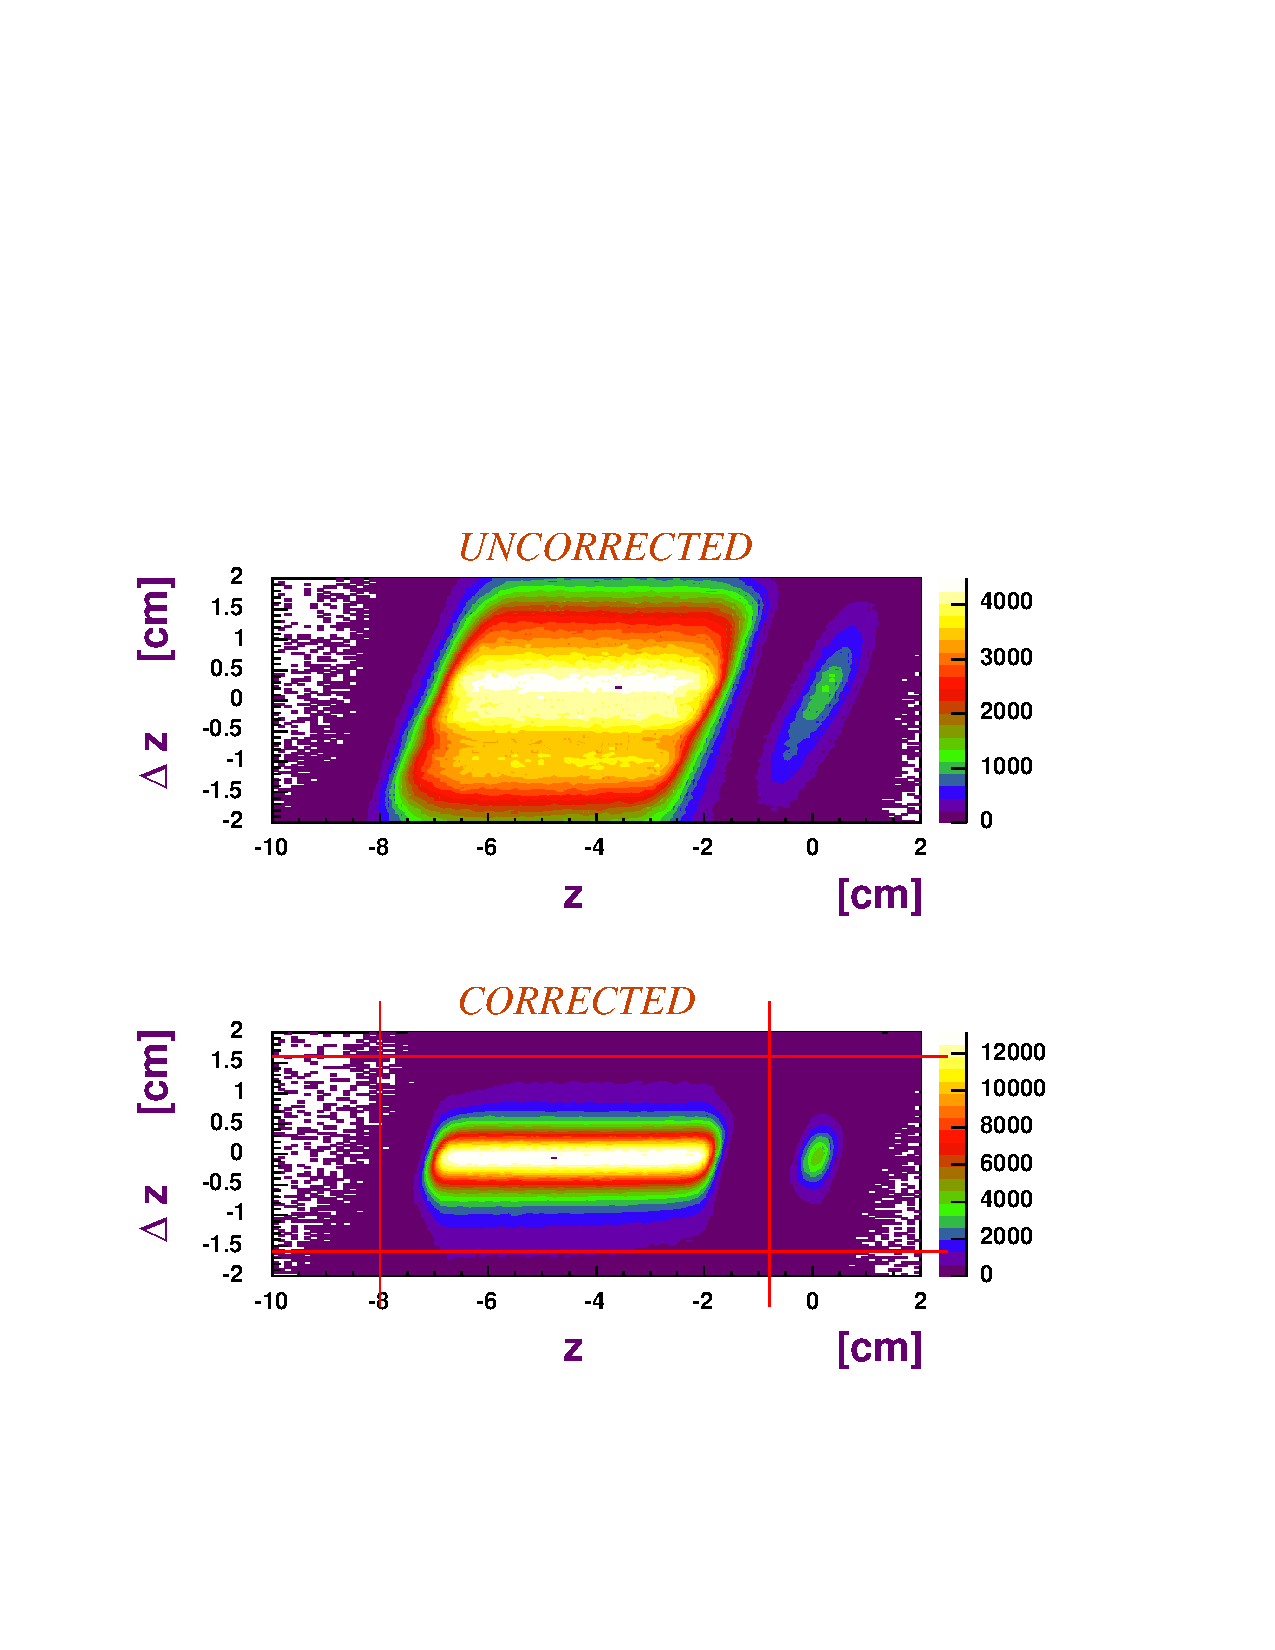
\includegraphics[width=11cm, bb=50 120 520 580]{data_reduction/img/vertex_cut}
  \caption[$\Delta z$ versus $z_{electron}$ uncorrected (top) and corrected (bottom) for all sectors]
          { $\Delta z$ versus $z_{electron}$ uncorrected (top) and corrected (bottom)
                     for all sectors.            
                     The distortions disappear with the correction and the resolution improves. }
 \label{fig:vertex_cut}
  \end{center} 
\end{figure}



























